\documentclass[10pt]{beamer}
\usetheme[left]{AAUsidebar}

\usepackage[utf8]{inputenc}
\usepackage[T1]{fontenc}

\usepackage{helvet}
\usepackage{graphicx}
\usepackage{listings}
\usepackage{color}
\usepackage[spanish]{babel}

\usepackage{subfigure}
\usepackage{ragged2e}

% colored hyperlinks
\newcommand{\chref}[2]{%
  \href{#1}{{\usebeamercolor[bg]{AAUsidebar}#2}}%
}

\title[Model-Based Quality Management
of Software Development Projects]% optional, use only with long paper titles
{Model-Based Quality Management
of Software Development Projects}

\subtitle{Administracion de modelos orientados la calidad de los proyectos de desarrollo de software}  % could also be a conference name

\date{\today}

\author[Raul Alejandro Buitrago Castellanos] % optional, use only with lots of authors
{
  Raul Alejandro Buitrago Castellanos\\
  \href{mailto:raulhabits@gmail.com}{{\tt raulhabits@gmail.com}}
}

\institute[
  Maestr\'ia en ciencias de la informaci\'on y las comunicaciones, con enfasis en ingenier\'ia de software\\
  Universidad Distrital Francisco Jose de Caldas\\
  Colombia
]
{
  Maestr\'ia en ciencias de la informaci\'on y las comunicaciones, con enfasis en ingenier\'ia de software\\
    Universidad Distrital Francisco Jose de Caldas\\
  Colombia
  
  %there must be an empty line above this line - otherwise some unwanted space is added between the university and the country (I do not know why;( )
}



\pgfdeclareimage[height=1.5cm]{titlepagelogo}{AAUgraphics/aau_logo_new} 
\titlegraphic{
  \pgfuseimage{titlepagelogo}
}


\begin{document}
{\aauwavesbg%
\begin{frame}[plain,noframenumbering] 
  \titlepage
\end{frame}}

% TOC
\begin{frame}{Agenda}{}
\tableofcontents
\end{frame}
%%%%%%%%%%%%%%%%

 \justifying

\section{Introducci\'on}
% motivation for creating this theme
\begin{frame}{Introducci\'on}{}

 "Managing the quality of artifacts created during the development process is an integral part of software project management."
\end{frame}
%%%%%%%%%%%%%%%%

\section{Consideraciones}
% motivation for creating this theme
\begin{frame}{Consideraciones}{}
 \justifying
 La administraci\'on y el control de los proyectos de desarrollo de software esta relacionada directamente tanto con la funcionalidad y el alcance del proyecto previamente establecidos; normalmente se ve reflejado en los siguientes aspectos.
 
 \begin{enumerate}
  \item {\tt Gesti\'on del costo} 
  \pause
  \item {\tt Gesti\'on del tiempo, y}
  \pause
  \item {\tt Gesti\'on de la calidad}
  \end{enumerate}
\end{frame}
%%%%%%%%%%%%%%%%

\section{Normas b\'asicas}
% the license
\begin{frame}{Normas b\'asicas}
 \begin{enumerate}
  \item {\tt Modelo de calidad del software ISO/IEC standard 9126-1 (2001)} 
  \pause
  \item {\tt Estandar para la evaluacion de productos de software ISO/IEC 14598-1 (1999)}
    \begin{enumerate}
     \item {\tt Calidad interna} 
     \item {\tt Calidad externa}
     \item {\tt Calidad en el uso}
     \end{enumerate}
  \pause
  \item {\tt Requerimientos y evaluaci\'on de la calidad de productos de software (SQuaRE) (ISO/IEC 25000-1 2005)}
  \end{enumerate}
\end{frame}
%%%%%%%%%%%%%%%%

\subsection{Selecci\'on de los modelos de calidad}
\begin{frame}{Selecci\'on de los modelos de calidad}
 Identificar el modelo que m\'as se ajusta y puede ser aplicado teniendo en cuenta el contexto. 
 \begin{enumerate}
  \item {\tt Que partes del proceso se deben analizar (artefactos)} 
  \item {\tt El proposito del modelo}
  \item {\tt Caracteristicas de inter\'es} 
  \item {\tt El proposito del modelo}  
  \item {\tt Selecci\'on del modelos m\'as adecuado}   
 \end{enumerate}
\end{frame}
%%%%%%%%%%%%%%%%
\subsection{Construcci\'on de modelos de calidad adaptados a las necesidades}
\begin{frame}{Construcci\'on de modelos de calidad adaptados a las necesidades}
 En \'algunas ocasiones no es viable el uso de un modelo en particular, por lo tanto se puede construir un modelo a partir de otros ya existentes.
 \begin{enumerate}
  \item {\tt Caracterizar,} 
  \item {\tt Definir los objetivos,}
  \item {\tt Escoger los procesos,} 
  \item {\tt Ejecutar,}  
  \item {\tt Seleccionar los modelos m\'as adecuados,}  
  \item {\tt Analizar, y}  
  \item {\tt Empaquetar.}  
 \end{enumerate}
\end{frame}
%%%%%%%%%%%%%%%%
\subsection{Especificaci\'on y aplicaci\'on de modelos de calidad}
\begin{frame}{Especificaci\'on y aplicaci\'on de modelos de calidad}
Modelo basado en el metamodelo de los procesos y los modelos de calidad.

\begin{figure}
\centering
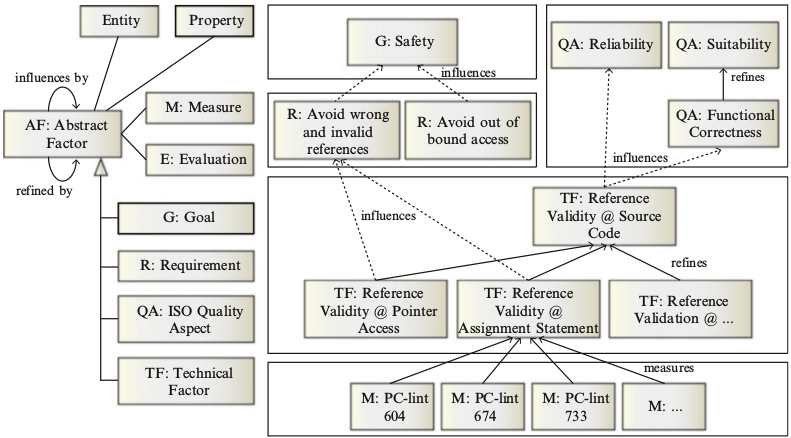
\includegraphics[width=0.7\linewidth]{./AAUgraphics/model_based_quality}
\caption{Ejemplo propuesto por el libro describiendo el metamodelo para los sistemas embebidos de una organizaci\'on}
\label{fig:model_based_quality}
\end{figure}

\end{frame}
%%%%%%%%%%%%%%%%
%%%%%%%%%%%%%%%%%%%%%%
\section{Conclusiones}
 \begin{frame}{Conclusiones}{}
 \justifying
 \begin{block}{}
  \begin{enumerate}
   \item {\tt La calidad es poco tangible en las fases iniciales de los procesos de desarrollo y por ende es dificil de medir objetivamente}
   \item {\tt A pesar que hay estandares, no existe una formula o un modelo que mencione la forma correcta para hacer el seguimiento y control el plan de calidad, y las actividades asociadas al aseguramiento de la misma; puesto que depende del contexto y la naturaleza del proyecto, entre otros.}
  \end{enumerate}
 \end{block}
 \end{frame}

%%%%%%%%%%%%%%%%%%%%%%
\section{Referencias}
\begin{frame}{Referencias}
 \begin{thebibliography}{1}
  \bibitem{knitr-book} Ruhe, Gunter and Wohlin, Claes. Software project management in a changing world. Springer. 2014.  
  \bibitem{latex-book} DE CASTRO KORGI, Rodrigo. El universo LATEX. Facultad de ciencias. Universidad Nacional de Colombia. Segunda edicion. 2003.  
 \end{thebibliography} 
\end{frame}

{\aauwavesbg
\begin{frame}[plain,noframenumbering]
  \finalpage{Gracias}
\end{frame}}
%%%%%%%%%%%%%%%%

\end{document}
